\documentclass[a4paper,12pt]{report}
\usepackage{graphicx}
\usepackage[utf8]{inputenc}
\begin{document}
\title{COP290 \\ Assignment 1 : Bubble Screensaver}
\author{Manoj Kataria\and Rohit\and Harishchandra Patidar}
\maketitle

\newpage
\tableofcontents
\newpage

\chapter{Introduction}
In this assignment, we were supposed to create a simple screen saver application. The application displays N balls on the screen. Each ball starts from a random position on the screen, and starts moving in a random direction. The collision of a ball with another ball, or the wall of the screen must be simulated using perfect reflection (no friction). Each ball on the screen is simulated by one thread. The collision between two balls must be simulated using messages between their respective threads. The speed of each ball can be increased/decreased by the user.
\chapter{Overall Design}
Given problem is broken into following components.
\begin{itemize}
\item[$\cdot$] GUI
\item[$\cdot$] Collisions
\item[$\cdot$] User Interface Controls
\item[$\cdot$] Multithreading
\item[$\cdot$] Utility Functions
\end{itemize}
These things are discussed in detail in the following chapters.
\chapter{Design Summary}
The entire application is divided into multiple files for different components and functions.\\\\
\textbf{Ball.h/.cpp}: Define Ball \\\\
\textbf{MyDefines.h}: All \#define directives defined here.\\\\
\textbf{MyEnum.h}: Enumeration utilities defined here\\\\
\textbf{global.h}: Structures Color and ThreeD defined here\\\\ 
\textbf{imageload.h/.cpp}: Contains Image class for BMP image.\\\\
\textbf{Particle.h/.cpp}: Contains class for snow particles.\\\\
\textbf{Theme.h/.cpp}: Contains Theme class\\\\ 
\textbf{themeReader.h}: Contains method to read themes.txt\\\\
\textbf{Wall.h/.cpp}: Contains wall class\\\\ 
\textbf{UtilityFunctions.h/.cpp}: Contains methods like Add/Remove ball etc.\\\\
\textbf{GUI.h/.cpp}: Contains all glut methods.\\\\  
\textbf{SubMenu.h/.cpp}: Contains UI control methods.\\\\    
\textbf{Collision.h/.cpp}: Contains method to handle collsions.
\chapter{GUI}
\section{Libraries included}
\begin{itemize}
\item[$\cdot$] GL/freeglut.h
\item[$\cdot$] GL/glui.h
\end{itemize}

\section{Camera Settings}
\begin{center}
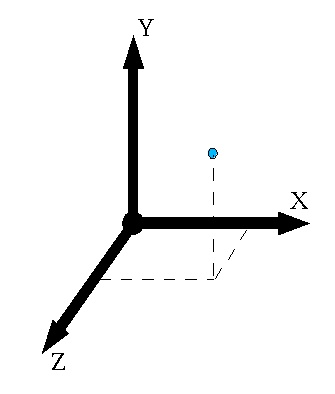
\includegraphics[height=5cm]{axis.png}\\
\end{center}
As positive z-axis points out of the screen and (0,0,0) lies in the plane of screen, therefore objects drawn on the screen are not visible. So firstly we shift the origin to (0,0,-zdistance) , where zdistance is shift in origin along negative z-axis and set camera angle to 90 degrees in y-direction.
\section{Resizing}
On reducing size of the window too much, at some stage the space required by balls is more than available window space. To avoid that we have set a limit on the size of the window. On reducing size below the limit, the view size does not decrease further.
\section{Drawing Balls}
\begin{center}
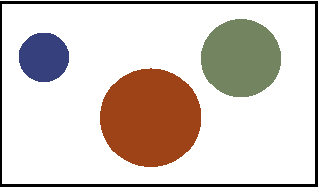
\includegraphics[height=5cm]{myballs.png}\\
\end{center}
We have set random radii of balls (\textit{in some particular range}) and given initial velocities in x and y directions such that no two balls overlap each other. To avoid overlapping while entering, we have used concept of timer such that new ball enters only when previous ball is far enough to avoid overlapping with this new ball. Each ball has a mass proportional to $(radius)^2$  assuming balls as disc in 2-Dimensional case (\textit{In case of 3d, mass is proportional to $(radius)^3$}). Also the color of balls are randomly generated. To display balls on the screen after regular interval of time  \textit{glutDisplayFunc()} and \textit{glutTimerFunc()} are used. The number of balls are entered by the user otherwise default number of balls are displayed on the screen.\\\\\\\\\\\\

\section{3D-View}

\begin{center}
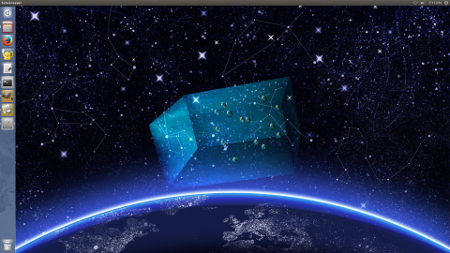
\includegraphics[height=5cm,width=10cm]{3d.png}\\
\end{center}
The application allows user to switch between 2D and 3D model. 3D model 
is the extension of 2D model. We have use Perspective model for both 3D and 2D model. In addition to x-y, spheres have also given velocities in z-direction. Following are the methods used to draw 3D-box and Spheres:
\begin{itemize}
\item[$\cdot$] glutSolidSphere
\item[$\cdot$] drawBox
\end{itemize}

\section{Textures}

To use textures in the application , we have defined class Image as following:
\textbf{Class Image:}\\\\
\hspace*{5mm}Member Variables:
\begin{itemize}
\item[$\cdot$] Data, Width , Height
\end{itemize}
In order to load BMP image we build method loadImage(). This method read BMP file and load it as Image. We have used these textures on spheres, faces of cube, backgrounds in the themes.

\section{Themes}
\begin{center}
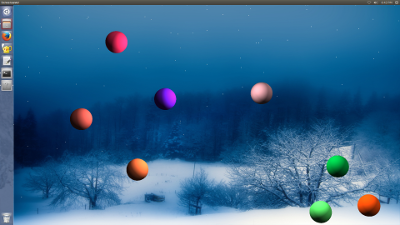
\includegraphics[height=5cm ,width=6cm]{t1.png}
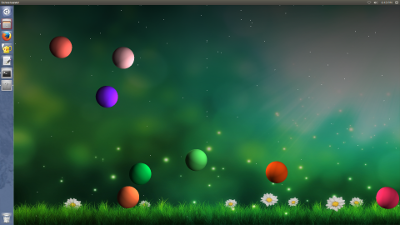
\includegraphics[height=5cm, width=6cm]{t2.png}
\end{center}\\
\begin{center}
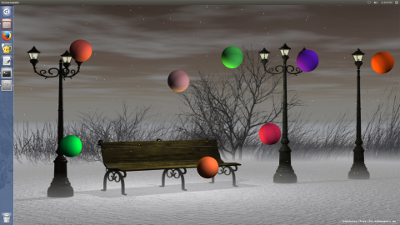
\includegraphics[height=5cm, width=6cm]{t3.png}
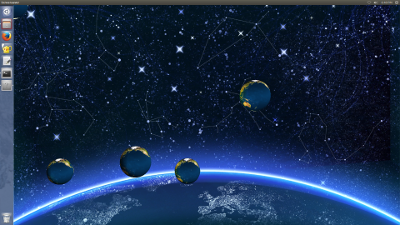
\includegraphics[height=5cm, width=6cm]{t4.png}
\end{center}\\\\
We have made our application cooler by adding various themes to it. Each theme has different light sources and background. Light sources will be enabled/disabled depending on the theme. Theme class is defined as following:\\
\textbf{Class Image:}\\\\
\hspace*{5mm}Member Variables:
\begin{itemize}
\item[$\cdot$] Background Color  
\item[$\cdot$] Image  
\item[$\cdot$] Light Sources  
\end{itemize}
The information about the colors and positions of light sources, backgrounds are stored in the text file. Theme reader method reads this information and provide it to the the theme class.

\chapter{Collisions}
\section{Ball to ball collision}
\subsection*{Condition for collision}
The distance between centers of two balls should be less than or equal to sum of their radii and they should be approaching each other.
\subsection*{Collision Mechanism}
\begin{center}
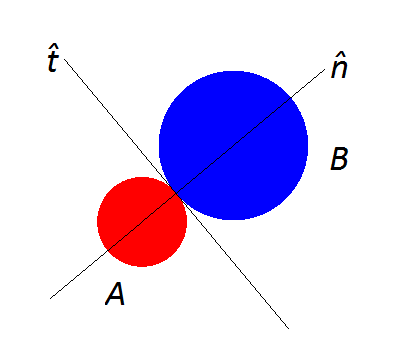
\includegraphics[height=5cm]{collision.png}\\
\end{center}
($x_{1},y_{1}$) = Center of ball A\\ 
($x_{2},y_{2}$) = Center of ball B\\
$m_{1}$ = Mass of ball A\\
$m_{2}$ = Mass of ball B\\
$\vec{u_{1}} \;= u_{x_{1}}\hat{i} + u_{y_{1}}\hat{j}$, Initial velocity of ball A\\
$\vec{u_{2}} \;= u_{x_{2}}\hat{i} + u_{y_{2}}\hat{j}$, Initial velocity of ball B\\
$\vec{v_{1}} \;= v_{x_{1}}\hat{i} + v_{y_{1}}\hat{j}$, Initial velocity of ball A\\
$\vec{v_{2}} \;= v_{x_{2}}$ $\hat{i}$ + $v_{y_{2}}$ $\hat{j}$, Initial velocity of ball B\\
$x \;= x_{2} - x_{1}$\\
$y \;= y_{2} - y_{1}$\\\\
$\hat{t}$ = $\frac{y\hat{i}-x\hat{j}}{\sqrt{x^{2}+y^{2}}}$ Unit vector normal to line of Impulse\\\\
$\hat{n}$ = $\frac{x\hat{i}+y\hat{j}}{\sqrt{x^{2}+y^{2}}}$ Unit vector along the line of impulse\\\\
When the two balls collide elastically, the change in their velocities is only due to change along $\hat{n}$ while velocities along $\hat{t}$ remain same i.e.\\\\
(1)\hspace*{3cm}$v_{1}\hat{t}$ = $u_{1}\hat{t}$\\\\
\textbf{Using conservation of momentum along the $\hat{n}$}\\\\
(2)\hspace*{3cm}$m_{1}\vec{u_{1}}\cdot\hat{n}+m_{2}\vec{u_{2}}\cdot\hat{n} = m_{1}\vec{v_{1}}\cdot\hat{n}+m_{2}\vec{v_{2}}\cdot\hat{n}$\\\\
\textbf{Using coefficient of restitution}\\\\
(3)\hspace*{3cm}e = $\frac{Velocity \; of\; approach}{Velocity\; of\; separation}$\\\\
As the collision is elastic, therefore e = 1. \\\\ 
Velocity of approach = Velocity of separtion i.e.
$\vec{u_{1}}\cdot\hat{n}-\vec{u_{2}}\cdot\hat{n} = -\vec{v_{1}}\cdot\hat{n}+\vec{v_{2}}\cdot\hat{n}$\\\\
\textbf{Using (2) and (3)}\\\\
(4)\hspace*{3cm}$\vec{v_{1}}\cdot\hat{n} = \frac{2*m_{2}u_{2}\cdot\hat{n} + (m_{1}-m_{2})u_{1}\cdot\hat{n}}{m_{1}+m_{2}}$\\\\
\textbf{Using (1) and (4)}\\\\
$v_{x_{1}} = \frac{y*(u_{x_{1}}y-u_{y_{1}}x)(m_{1}+m_{2}) + x*[(m_{1}-m_{2})(v_{x_{1}}x+v_{y_{1}}y)+2m_{2}(v_{x_{2}}x+v_{y_{2}}y)]}{(x^{2}+y^{2})(m_{1}+m_{2})}$\\\\
$v_{y_{1}} = \frac{x*(u_{y_{1}}x-u_{x_{1}}y)(m_{1}+m_{2}) + y*[(m_{1}-m_{2})(v_{y_{1}}y+v_{x_{1}}x)+2m_{2}(v_{y_{2}}y+v_{x_{2}}x)]}{(x^{2}+y^{2})(m_{1}+m_{2})}$\\\\
For ball B replace x by -x and y by -y.\\

\section{Ball to wall collision}

\begin{center}
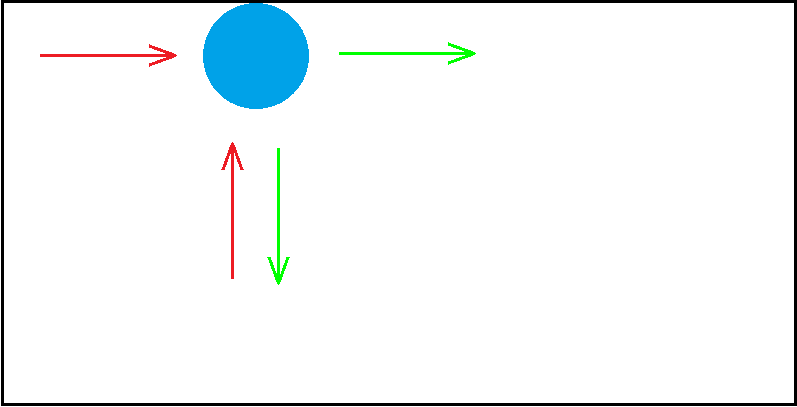
\includegraphics[height=5cm,width=10cm]{WallCollision.png}\\
\end{center}
Collision with Left/Right wall:\\
$v_{x} = -u_{x}$\\\\
Collision with Upper/Lower wall:\\
$v_{y} = -u_{y}$
\\\\\\
\textbf{In case of 3D, the above formula can be extended accordingly.}

\chapter{User Interface Controls}

\section{Menu controls}
To use various features of the application we have created GLUI  window. This window has following controls in it:
\begin{center}
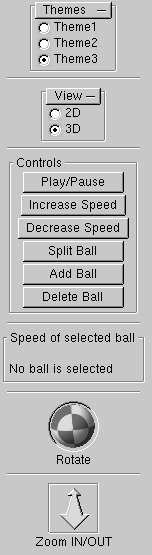
\includegraphics[height=7cm,width=2cm]{menu.png}\\
\end{center}
\begin{itemize}
\item[$\cdot$] Themes
\item[$\cdot$] Views (2D/3D)
\item[$\cdot$] Increase/Decrease Speed
\item[$\cdot$] Display speed of the selected ball
\item[$\cdot$] Add a ball
\item[$\cdot$] Remove the selected ball
\item[$\cdot$] Split the selected ball
\item[$\cdot$] Rotate/Translate 3D box
\end{itemize}
\section{Key Events:}
User can control motion of selected ball using key buttons.\\\\
\textbf{w Key} : Increase speed in positive-y direction\\
\textbf{s Key} : Increase speed in negative-y direction\\
\textbf{a Key} : Increase speed in negative-x direction\\
\textbf{d Key} : Increase speed in positive-x direction\\
\textbf{Esc Key} : Exit the application\\\\
\section{Mouse Events:}
To select the particular ball user can click on it using the mouse. On clicking the border appears on the selected ball. After selection user can use features provided in the control menu.

\chapter{Multithreading}
\section{N threads managing N balls}
\subsection*{Method I}
Balls are maintained in a global vector. Each of the N threads checks for possible collisions of a \textit{ball} (ID of which is passed to it as argument) with all the other balls. Each thread keeps track of change in velocity of \textit{ball} in a variable \textit{dv}(member variable of Ball Class). Threads do not change/set the velocities or any other attribute of \textit{ball} passed to it. All changes are made outside the threads (in main or any other update function using dv of ball) after all threads are finished (this is accomplished by joining all threads to main thread). Since threads just check for possible collisions of balls in parallel and no changes are made to global vector of balls from inside the threads, mutexes are not required for this purpose.
\subsection*{Method II}
In this method, we define our own thread class \textbf{MyThread}\\\\
Class \textbf{MyThread} \{\\
\hspace*{1cm} Ball \textbf{B};\\
\hspace*{1cm} queue$<$*Ball$>* q$;\\\\
\}\\\\
We have a vector \textit{threads} of MyThread objects which is in global scope and is initially empty. When a new ball is required, a MyThread object is created and pushed into the vector.
\\
At each \textit{update()} call , \textit{addWorkItems()} method is called which adds to the queue of each thread,pointers to ball object of other threads.
\\
All the threads then run in parallel, successively checking collisions with others balls in its queue and removing them after updating their velocities accordingly.
\\
Each Ball has a mutex associated with it, which is locked whenever accessing/setting its attributes thereby in synchronization with other threads.
\chapter{Testing Components}
\section{Collision}
\begin{enumerate}
\item[$\cdot$] To verify that collisions between the balls are proper, we output the kinetic energy of system in a log file. Since the collisions are elastic therefore kinetic energy of the system will remain conserved at all time. (unless user increases or decreases the speed of any ball)
\item[$\cdot$] To test collision of a ball with wall, set velocity only in one direction(x or y) and then check with a random velocity.
\item[$\cdot$] To test collision of a ball with another ball, first test head on collision in both x and y direction and check collisions at different angles. Using GDB and setting breakpoints at the time of collision we can check whether the balls are overlapping or not. 
\item[$\cdot$] To test collision of multiple balls simultaneously, although a rare event in random case, take 3 balls at vertices of a equilateral triangle and give them velocities toward the centroid of triangle.
\end{enumerate}
\section{Multithreading}
Whether all the threads are running or not can be tested in GDB by setting breakpoints at different function calls.

\end{document}
